\section{Relação Rastreamento e Reconhecimento}
\label{sec:rastreamento-reconhecimento}

	Até agora, foi mostrado como os Módulos de Rastreamento e de Reconhecimento funcionam de maneira isolada, mas não como se relacionam. O Módulo de Rastreamento detém as informações sobre todos os usuários rastreados no ambiente e é responsável por requisitar reconhecimento ao Módulo de Reconhecimento, que deverá acontecer quando um novo usuário for detectado ou quando for necessário reconhecer um usuário já rastreado.

	Basicamente, quando um novo usuário for detectado, a relação entre rastreamento e reconhecimento acontecerá de acordo com as etapas descritas na Figura~\ref{fig:rastreamento-reconhecimento}.

		\begin{figure}[hbt]
			\begin{center}
				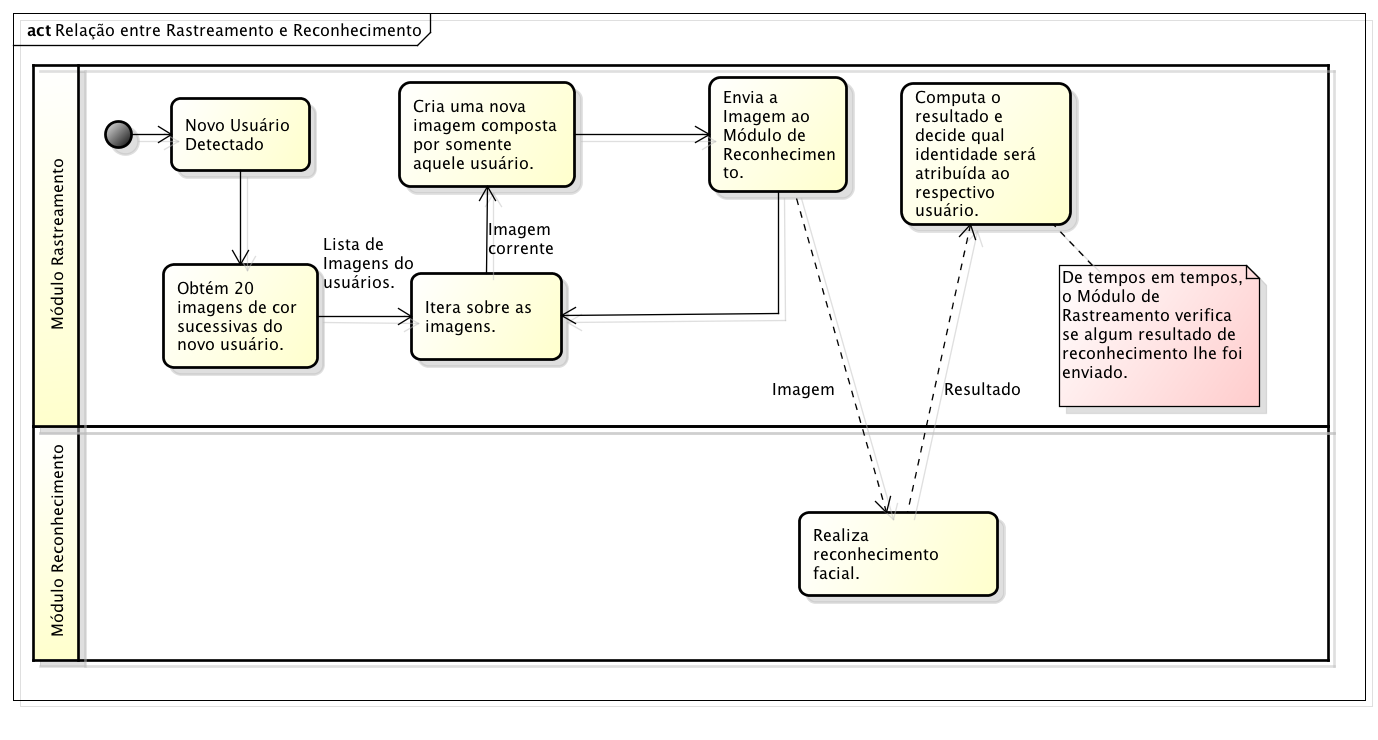
\includegraphics[scale=0.6]{figuras/4.ProblemaEProposta/diagrama-relacao.png}
			\end{center}
			\caption{Representação da relação que o Módulo de Rastreamento terá com o Módulo de Reconhecimento quando um novo usuário for detectado.}
			\label{fig:rastreamento-reconhecimento}
		\end{figure}
	
		% \begin{enumerate}
		%  	\item O Módulo de Rastreamento detecta novo usuário, e obtém um número pré-definido de imagens sucessivas do novo usuário. Para cada imagem, ele cria uma nova imagem de cor contendo somente aquele usuário, como mostrado na Figura (\textbf{colocar a figura aqui}), e a envia para o Módulo de Reconhecimento.
		%  	\item Para cada imagem recebida, o Módulo de Reconhecimento tenta reconhecer o novo usuário e retorna ``vazio'' ou o nome e a confiança do reconhecimento.
		%  	\item O Módulo de Rastreamento verifica se a confiança é maior que um limiar pré-definido, se for ele incrementa o contador que armazena o número de vezes que o usuário foi reconhecido, armazena o nome obtido juntamente com a confiança e calcula qual nome  será atribuído ao novo usuário. Esse cálculo será feito por meio de uma média ponderada utilizando os diferentes resultados obtidos por cada reconhecimento e suas respectivas confianças.
	 % 	\end{enumerate} 
	
	Ao invés de tentar realizar o reconhecimento somente quando novos usuários são detectados, o Sistema TRUE continua a tentar reconhecer os usuários já reconhecidos para melhorar a confiança no reconhecimento. Essas tentativas de reconhecer novamente os usuários ocorrerão em intervalos de tempo pré-definidos seguindo as mesmas etapas de quando um novo usuário for detectado. A única etapa que se difere é a primeira: ao invés de obter várias imagens de um mesmo usuário, são obtidas uma imagem de cada usuário rastreado e as mesmas são enviadas ao Módulo de Reconhecimento.

	Como visto na Figura~\ref{fig:rastreamento-reconhecimento}, ao obter um resultado de reconhecimento para determinado usuário, o Módulo de Rastreamendo deve computar qual identidade será atribuída ao mesmo. Para isso, este módulo mantém para cada usuário o número total de vezes que já foi reconhecido, os diferentes nomes obtidos pelo Módulo de Reconhecimento bem como a confiança média para cada nome e o número de vezes que cada nome foi atribuído ao usuário. Com todos esses dados, a identidade do usuário é escolhida por meio de uma média ponderada entre as confianças de cada nome onde os pesos utilizados são compostos pelo número de vezes que o respectivo nome foi atribuído ao usuário. Vejamos o seguinte exemplo para ilustrar esse cálculo:

	\begin{description}
		Seja João um usuário do ambiente inteligente que está sendo rastreado a algum tempo e que já foi reconhecido algumas vezes. No momento, o Módulo de Rastreamento mantém vários dados sobre o João descritos na Tabela~\ref{tab:joao}. Então, para computar qual identidade será atribuída ao usuário, o Módulo de Rastreamento realiza os cálculos~\ref{eq:joao}. Como o resultado da média ponderada se aproxima mais da confiança do nome João, este foi escolhido como sendo sua identidade.
	\end{description}

	\begin{table}[H]
		\begin{center}
			\caption{Exemplos de dados de reconhecimento mantidos para cada usuário rastreado pelo Módulo de Rastreamento.}
			\begin{tabular}{|c|c|c|}
				\hline \bf Nome & Confiança Média & Número de Vezes \\
				\hline \hline \bf João & 0.947302 & 15 \\
				\hline \bf  Danilo & 0.934010 & 1 \\
				\hline \bf Tales & 0.950320 & 3 \\
				\hline
				\hline \multicolumn{2}{|c|}{\bf Total}  & 19 \\
				\hline
			\end{tabular}
		\end{center}
		\label{tab:joao}
	\end{table}

	\begin{align}
		\label{eq:joao}
		M_p = \frac{15 * 0.947302 + 1 * 0.934010 + 3 * 0.950320}{19} = 0.947079
	\end{align}

	\begin{align}
	\nonumber & Joao: 0.947079 - 0.947302 = -0.000223\\
		\nonumber & Danilo: 0.934010 - 0.947302 = -0.013292\\
		\nonumber & Tales: 0.950320 - 0.947302 = 0.003018
	\end{align}

	Com todos esses dados de reconhecimento, além dos dados de rastreamento e localização de cada usuário, o Módulo de Rastreamento consegue centralizar todas as informações necessárias de cada usuário. A Figura~\ref{fig:truetotal} exemplifica um usuário rastreado pelo Sistema TRUE onde as informações de localização e identificaçao estão presentes.

	% FIGURA usuario rastreado, localizado e identificado

